\documentclass[conference]{IEEEtran}
%\IEEEoverridecommandlockouts
% The preceding line is only needed to identify funding in the first footnote. If that is unneeded, please comment it out.
\usepackage{cite}
\usepackage{amsmath,amssymb,amsfonts}
\usepackage{algorithmic}
\usepackage{graphicx}
\usepackage{textcomp}
\usepackage{xcolor}
\usepackage{booktabs}                        % AAB inserido
\usepackage[utf8]{inputenc}                  % AAB inserido
\usepackage{rotating}                        % AAB inserido
%\usepackage{subfigure}                       % AAB inserido
%\usepackage[export]{adjustbox}               % AAB inserido
\usepackage{bbm}

\ifCLASSOPTIONcompsoc                        % AAB inserido
\usepackage[caption=false,font=normalsize,labelfont=sf,textfont=sf]{subfig}
\else
\usepackage[caption=false,font=footnotesize]{subfig}
\fi
%\usepackage[round,sort,nonamebreak]{natbib}  % AAB inserido
%\usepackage[round,sort,nonamebreak]{natbib} % citação bibliográfica textual
\def\BibTeX{{\rm B\kern-.05em{\sc i\kern-.025em b}\kern-.08em
    T\kern-.1667em\lower.7ex\hbox{E}\kern-.125emX}}
%AAB
\DeclareMathOperator{\traco}{tr}
\graphicspath{{../../Dissertacao/figuras/}}
\begin{document}

\title{Fusion of Evidences for Edge Detection in PolSAR Images\\
%{\footnotesize \textsuperscript{*}Note: Sub-titles are not captured in Xplore and
%should not be used}
\thanks{Grantee Capes/PROSUP/Mackenzie.}
}
\author{\IEEEauthorblockN{Anderson A.\ de Borba}
\IEEEauthorblockA{\textit{Dept.\ Engenharia Elétrica e Computação} \\
\textit{UPM -- Universidade Presbiteriana Mackenzie}\\
IBMEC-SP\\
São Paulo, Brazil \\
anderson.borba@ibmec.edu.br}
\and
\IEEEauthorblockN{Maurício Marengoni}
\IEEEauthorblockA{\textit{Dept.\ Engenharia Elétrica e Computação} \\
\textit{UPM -- Universidade Presbiteriana Mackenzie}\\
São Paulo, Brazil \\
mauricio.marengoni@mackenzie.br}
\and
\IEEEauthorblockN{Alejandro C.\ Frery}
\IEEEauthorblockA{Laboratório de Computação Científica e Análise Numérica -- LACCAN} \\
\textit{UFAL -- Universidade Federal de Alagoas}\\
Maceió, Brazil \\
acfrery@laccan.ufal.br}
\maketitle
\begin{abstract}
Polarimetric Synthetic Aperture Radar (PolSAR) has achieved an important position as a remote sensing imaging method. 
However, PolSAR images are contaminated with speckle noise, making its processing and analysis challenging tasks. 
The present study discusses a detection method based on the fusion of evidences obtained in the intensity channels of multilook PolSAR images.
The method consists of detecting transition points in the finest strip of data which spans two regions using the maximum likelihood.
This is applied to each of the three intensity channels (hh), (hv) and (vv). 
The fusion methods are simple average, stationary wavelet transform (SWT), principal component analysis (PCA) and ROC statistics.  
%%% Esperar o artigo ficar pronto e pontuar o que foi feito
The results indicate improvement performance of the approach in detecting edges with possible paths for future research.
\end{abstract}

\begin{IEEEkeywords}
PolSAR, edge detection, maximum likelihood estimation, fusion
\end{IEEEkeywords}

\section{Introduction}\label{sec_01}

This work presents results on the detection and fusion of edge evidence applied to Polarimetric Synthetic Aperture Radar images (PolSAR). Models and algorithms as required for an appropriate treatment of their special statistical characteristics were employed.

Among the available edge detection techniques for SAR imagery, it is worth mentioning those based on the gradient, Refs.~\cite{tlb, obw, flmc, fyf}, and on Markov chains, Ref.~\cite{bf}. The former suffer from the effect of speckle, and the latter lead to computer intensive methods. Ref.~\cite{gfn} presents a comparison between several edge detectors. 

Alternatively, techniques based on statistical modeling have been used in edge detection, Refs.~\cite{gmbf, fbgm, horrit, gfn} and, more recently, by means of \textit{Deep Learning}, Refs.~\cite{bac, ztmxzxf, tabmm, xstz}.

This work relies on ideas stemming from information fusion.
This approach has been followed by Refs.~\cite{sglmla,sg} in order to extract valuable knowledge from remotely sensed data.

This paper follows the statistical modeling approach, mainly the techniques described in Refs.~\cite{fbgm, nhfc} using the Wishart distribution.
The basis for the fusion of information is described in Refs.~\cite{mit, sg}. 

The objective of this work yo show the viability of a procedure to detect edges in each channel of a PolSAR image and to perform the fusion of the edge evidence, with the task of understanding and quantifying the importance of the information provided by each channel in order to provide a better detection.

The article is structured as follows: 
Section~\ref{sec_02} describes the statistical modeling for PolSAR data, 
its use is presented in Sections~\ref{sec_03}, \ref{sec_04}, ~\ref{sec_05}, and~\ref{sec_06}.
Section~\ref{sec_07} describes the fusion of edge evidence approaches with an emphasis on the ROC statistics-based method.
Numerical results are shown and analyzed in Section~\ref{sec_08} and, finally, Section~\ref{sec_09} concludes the paper with remarks, future research directions and the viability  to detect edges in each channel of a PolSAR image.

\section{Statistical modeling for PolSAR data}\label{sec_02}

Fully polarimetric SAR systems transmit orthogonally polarized microwave pulses and measure orthogonal components of the received signal. 
For each pixel, we have a matrix of scattering coefficients, which are complex numbers and describe the transformation from the transmitted electromagnetic field to the received electromagnetic field.

The transformation can be represented as
\begin{equation*}
 \left[
\begin{array}{c}
	E_{\text{h}}^{\text{r}}   \\
	E_{\text{v}}^{\text{r}}    
\end{array}
\right]
 = \frac{e^{\hat{\imath} kr}}{r}\left[
\begin{array}{cc}
	S_\text{hh}   & S_\text{hv}   \\
	S_\text{vh}   & S_\text{vv}   
\end{array}
\right]
 \left[
\begin{array}{c}
	E_{\text{h}}^{\text{t}}   \\
	E_{\text{v}}^{\text{t}}    
\end{array}
\right],
\end{equation*}
where $k$ denotes the wave number, $\hat{\imath}$ is the complex unit, and $\text{r}$ is the distance between the radar and the target. 
The electromagnetic field with components $E_{\text{i}}^{\text{j}}$ has a subscribed index denoting horizontal ($\text{h}$) or vertical ($\text{v}$) polarization, while the superscript index indicates the received ($\text{r}$) or transmitted ($\text{t}$) wave. 
Defining $S_\text{ij}$ as the complex scattering coefficients, such that the indexes $\text{i}$ and $\text{j}$ are associated with the reception and transmission of waves, for example, the scattering coefficient $S_\text{hv}$ is associated with wave transmitted in the vertical direction ($\text{v}$) and received in the horizontal direction ($\text{h}$).

The complex scattering matrix $\mathbf{S}$ is defined by
\begin{equation}
\mathbf{S} = \left[
\begin{array}{cc}
	S_\text{hh}   & S_\text{hv}   \\
	S_\text{vv}   & S_\text{vv}   
\end{array}
\right],
\label{eq_01}
\end{equation}
and if the means of propagation of waves is reciprocal, then the reciprocity theorem, Ref.~\cite{lp}, allows us to state the scattering matrix as being Hermitian. 
In this way, the scattering matrix~(\ref{eq_01}) can be represented by the vector $\mathbf{s}=[S_\text{hh},S_\text{hv},S_{\text{vv}}]^T$.

Following Refs.~\cite{good, lee}, we will assume that the distribution of $\mathbf{s}$ is Gaussian circular complex multivariate with zero mean $N^{\mathbbm C}_3(0,\mathbf{\Sigma})$, and probability density function (pdf) given by:
\begin{equation}
    f_{\mathbf{s}}(\mathbf{s};\mathbf{\Sigma})=\frac{1}{\pi^3|\mathbf{\Sigma}|} \exp(-\mathbf{s}^H\mathbf{\Sigma}^{-1}\mathbf{s}),
    \label{eq_02}
\end{equation}
where $|\cdot|$ is the determinant, 
the superscript index $H$ denotes the conjugate complex number, 
and $\mathbf{\Sigma}$ is the covariance matrix of $\mathbf{s}$ such that $\mathbf{\Sigma}=E[\mathbf{ss}^H]$, where $E[\cdot]$ denotes the expected value. 

This statistical modeling has been confirmed for a variety of the polarimetric SAR data, and it contains all the necessary information to characterize the backscatter according to Refs.~\cite{sarabendi,mfp}
 
The statistical modelling described so far deals only with single-look modelling.
However, polarimetric images are usually subjected to a multi-look processing in order to improve the signal-to-noise ratio. 
For this purpose, Refs.~\cite{good, ade} show that estimated positive definite Hermitian matrices are obtained by computing the average of $L$ independent samples of the same scene, resulting in the estimated sample covariance matrix:
\begin{equation}
    \mathbf{Z}=\frac{1}{L}\sum_{\ell=1}^{L} {\mathbf{s}_\ell}{\mathbf{s}_\ell}^H,
    \label{eq_03}
\end{equation}
where $\mathbf{s}_\ell$, $\ell = 1, \dots, L$, are $L$ independent samples of complex vectors distributed as $\mathbf{s}$. 
The sample covariance matrix associated with $\mathbf{s}_\ell$ denotes the scattering for each of the $L$ looks.

\section{Multi-look Wishart density function}\label{sec_03}

Multi-looked data follow a Wishart distribution with probability density function defined by:
\begin{equation}
    f_{\mathbf{Z}}(\mathbf{Z};\mathbf{\Sigma_{s}},L)=\frac{L^{mL}|\mathbf{Z}|^{L-m}}{|\mathbf{\Sigma_{s}}|^{L}\Gamma_m(L)} \exp(-L\traco(\mathbf{\Sigma_{s}}^{-1}\mathbf{Z})),
    \label{eq_04}
\end{equation} 
where, $\traco(\cdot)$ is the trace operator of an array, $\Gamma_m(L)$ is a multivariate Gamma function defined by
\begin{equation*}
	\Gamma_m(L)=\pi^{\frac{1}{2}m(m-1)} \prod_{i=0}^{m-1}\Gamma(L-i),
\end{equation*}
and $\Gamma(\cdot)$ is the Gamma function.
In our study we will consider $m=3$. 
We denote this situation $\mathbf{Z}\sim W(\mathbf{\Sigma_{s}}, L)$, which satisfies $E[\mathbf{Z}]=\mathbf{\Sigma_{s}}$. 
Since there is no ambiguity, we will use $\mathbf{\Sigma}$ instead of $\mathbf{\Sigma_{s}}$ to represent the covariance matrix associated with $\mathbf{S}$.

\section{Edge Detection}\label{sec_04}

Most of the usual techniques for edge detection, e.g., 
Sobel, Canny, Laplacian of Gaussian (LoG) and pyramidal LoG, assume additive Gaussian noise and, thus, are ineffective for PolSAR imagery.
The noise in these kind of images is multiplicative, making edge detection in SAR images a challenging task.

The main idea for edge detection is based on Ref.~\cite{nhfc, gmbf} and show how to detect the transition point in a thin strip between two regions of the image. The transition point is considered as edge evidence. 

The following procedure is proposed:
\begin{enumerate}
	\item identify the centroid of a region of interest (ROI) in an automatic, semi-automatic or manual manner;
	\item cast rays from the centroid to the outside of the area;
	\item collect data around the rays using the  Bresenham's midpoint line algorithm, ideally the size of a pixel;
	\item detect points in the data strips which provide evidence of changes in their statistical properties, i.e., a transition point that defines edge evidence;
	\item use the Generalized Simulated Anneling (GenSA) method, Ref.~\cite{xgsh}, to find maximum points in the functions of interest;
	\item fuse the evidence of detected edges in the $\text{hh}$, $\text{hv}$ and $\text{vv}$ channels.
\end{enumerate}
With this, fully polarized data is not required, only the intensity channels.

\section{Maximum Likelihood Estimator (MLE)}\label{sec_05}

Suppose $\mathbf{X}=(X_1,X_2,\dots,X_n)^T$ is a random vector distributed according to the probability density function $f(\mathbf{x},\mathbf{\theta})$ with parameters $\mathbf{\theta}=(\theta_1,\dots,\theta_d)^T$ in the parameter space $\Theta$.
The likelihood function is
\begin{equation*}
    L(\theta;\mathbf{X}) = \prod_{i=1}^{n}f(x_i;\theta),
\end{equation*}
and the logarithmic likelihood function, which is also called the log-likelihood function is
\begin{equation}
	\ell(\theta;\mathbf{X})= \ln L(\theta;\mathbf{X}) = \sum_{i=1}^{n}\ln f(x_i;\theta).
	\label{eq_05}
\end{equation}

A maximum likelihood estimator is any point in $\Theta$ satisfying $\widehat{\theta}= \arg\max\limits_{\theta\in\Theta}L(\theta;\mathbf{x})$ or, equivalently, $\widehat{\theta}= \arg\max\limits_{\theta\in\Theta}\ell(\theta;\mathbf{x})$.

Consider now that the sample $\mathbf{Z}^T=(\mathbf{Z}_1,\mathbf{Z}_2,\dots,\mathbf{Z}_N)$ is split in two: $\mathbf{Z}_1,\dots,\mathbf{Z}_j$ and $\mathbf{Z}_{j+1},\dots,\mathbf{Z}_j$.
These parts may belong to two different Wishart distributions: those characterized by  $\mathbf{\Sigma_A}$, and $\mathbf{\Sigma_B}$, both with the same number of looks $L$.
Finding the edge consists in finding the point $j$ (or $j+1$) that separates them.

Finding the edge $j$ by maximum likelihood can be achieved by looking for the position $\widehat\jmath$  that maximizes the likelihood equation of the two samples:
%
\begin{equation}
	L(j)=\prod_{k_1=1}^{j}f_{\mathbf{Z}}(\mathbf{Z}_{k_1};\mathbf{\widehat\Sigma_{A}},L) \prod_{k_2=j+1}^{N}f_{\mathbf{Z}}(\mathbf{Z}_{k_2};\mathbf{\widehat\Sigma_{B}},L),
	\label{eq_06}
\end{equation}
where $\mathbf{\widehat\Sigma_{A}}$ is the maximum likelihood estimator of $\mathbf{\Sigma_{A}}$ based on the sample $\mathbf{Z}_1,\dots,\mathbf{Z}_{j}$, 
and $\mathbf{\widehat\Sigma_{B}}$ is the maximum likelihood estimator of $\mathbf{\Sigma_{B}}$ based on the sample $\mathbf{Z}_{j+1},\dots,\mathbf{Z}_{N}$.
Analogously, one may optimize with respect to $j$ the log-likely function, i.e., finding where
\begin{equation}
\ell(j) =
	\sum_{k_1=1}^{j}\ln f_{\mathbf{Z}}(\mathbf{Z}_{k_1}; \mathbf{\widehat\Sigma_{A}},L) + \sum_{k_2=j+1}^{N}\ln f_{\mathbf{Z}}(\mathbf{Z}_{k_2};     \mathbf{\widehat\Sigma_{B}},L).
	\label{eq_07}
\end{equation}
is maximum with respect to $1\leq j \leq N$.
The point that solves this optimization problem is denoted $\widehat{\jmath}$.
%$\widehat\jmath = \arg\max\limits_{1\leq \jmath\leq N}\ell(\jmath)$

The estimates for the covariance matrices can be found using the maximum likelihood estimator denoted by $\widehat{\Sigma}$, Ref.~\cite{good}: 
\begin{equation}
\widehat{\mathbf\Sigma_{I}}(j) = \left\{
\begin{array}{lc}
	j^{-1}\sum_{k=1}^{j}\mathbf{Z}_{k}  & \mbox{if}\quad I=A,  \\
        (N-j)^{-1}\sum_{k=j+1}^{N}\mathbf{Z}_{k} & \mbox{if}\quad I=B.
\end{array}
\right.\label{eq_08}
\end{equation}

After algebraic manipulations on each term of the summation using the equation~\eqref{eq_08}, we obtain
\begin{align}\nonumber
	\ell(j)&=N\left[mL(\ln{L}-1)-\ln{\Gamma_m(L)}\right]\\\nonumber
	&- L\left[j\ln{|\mathbf{\widehat{\Sigma}}_{A}(j)|} +(N-j)\ln{|\mathbf{\widehat{\Sigma}}_{B}(j)|}\right] \\
	&+ (L-m)\sum_{k=1}^{N}\ln{|\mathbf{Z}_{k}|}.\label{eq_09}
\end{align}

The argument of the maximum $\widehat{\jmath}$ is the edge evidence that will be used in our fusion methods.

\section{Application in simulated images}\label{sec_06}

The methodology (MLE) for detecting edge evidence will be applied to a simulated image based on Refs.~\cite{nhfc,gamf}. 
The image has $400\times400$ pixels and is composed of two samples obeying the Wishart distribution; cf.\ Fig.~\ref{fig_Edges-Evidence}\subref{fig_Edges-Evidence:a}.

For each pair of covariance matrices $\Sigma_{k_1}$, $\Sigma_{k_2}$ we simulate a PolSAR image $I_{k_1,k_2}$: 
samples of $W_G(\Sigma_{k_1}, 4)$ in the left half, and 
samples of $W_G(\Sigma_{k_2}, 4)$ in the right half.
The image has $400 \times 400$ pixels.

\begin{figure}[hbt]
     \subfloat[Pauli decomposition \label{fig_Edges-Evidence:a}]{%
       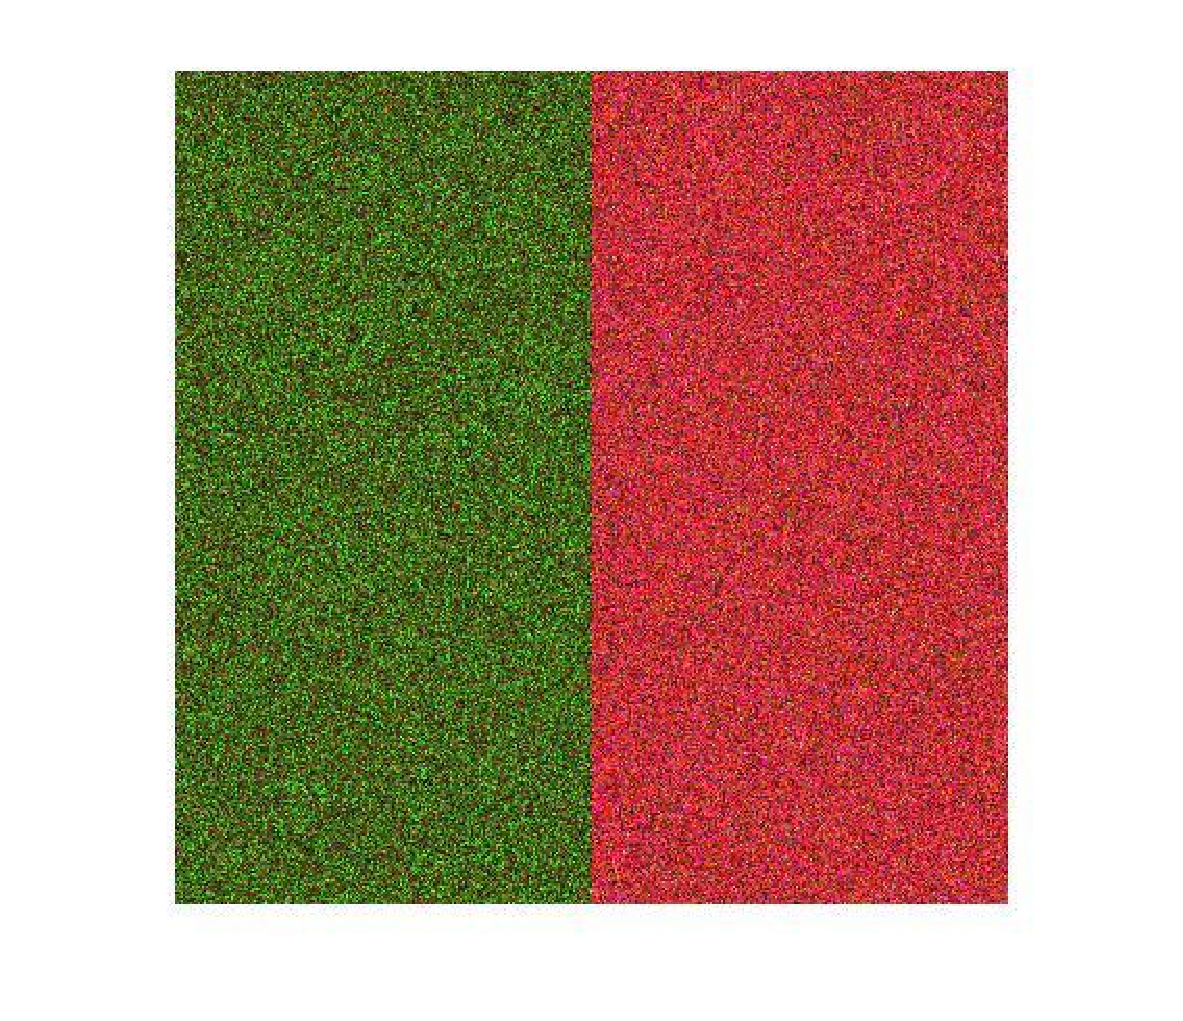
\includegraphics[viewport= 80 50 490 460, clip=true, width=0.23\textwidth]{phanton_nhfc_dec_pauli}}      
     \subfloat[Marginal densities of the $\text{hh}$ channel\label{fig_Edges-Evidence:b}]{%
       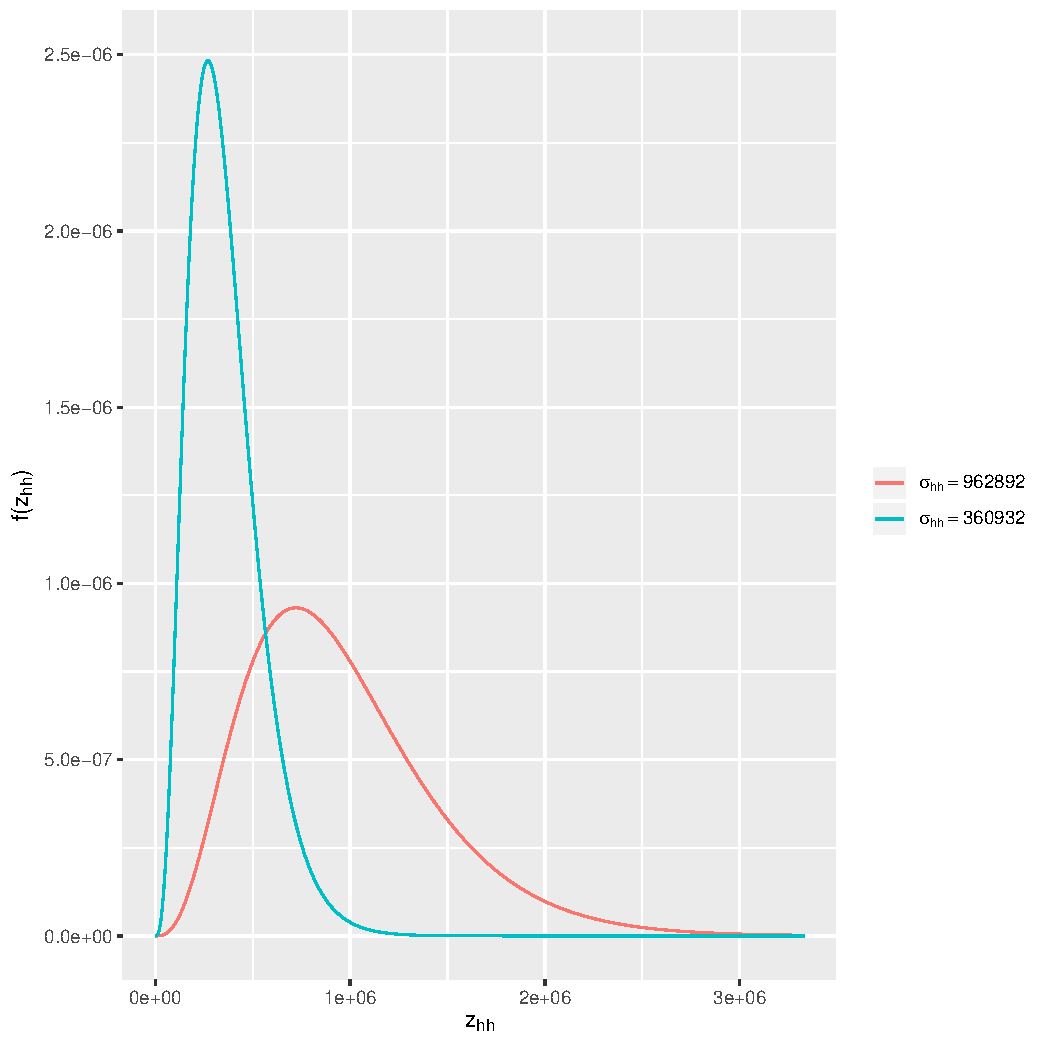
\includegraphics[width=0.24\textwidth]{grafico_pdf_nhfc_2014_sigma_hh_artigos}
     }
    \caption{Edges evidences}
     \label{fig_Edges-Evidence}
\end{figure}

The Pauli decomposition is based on the linear combination of intensity channels: $(\mathbf{I_\text{hh}+I_{\text{vv}}}, \mathbf{I_\text{hh}-I_{\text{vv}}}, \mathbf{I_\text{hv}})$. 
This decomposition is shown in Fig.~\ref{fig_Edges-Evidence}\subref{fig_Edges-Evidence:a}. 

Fig.~\ref{fig_Edges-Evidence}\subref{fig_Edges-Evidence:b}. 
shows the density function of $\sigma_\text{hh}$ with parameters extracted from real data for forest and urban areas: $\sigma_\text{hh}=962892$ and $\sigma_\text{hh}= 360932$.  

Fig.~\ref{fig_Edges-Evidence}~\subref{fig_Edges-Evidence:a} shows the evidence of edge in the middle line.
    
\begin{figure}[hbt]
	\centering
     \subfloat[Band $\text{hh}$ \label{fig_evid_bordas:1a}]{%
       %\includegraphics[width=0.2\textwidth]{example-image-a}
       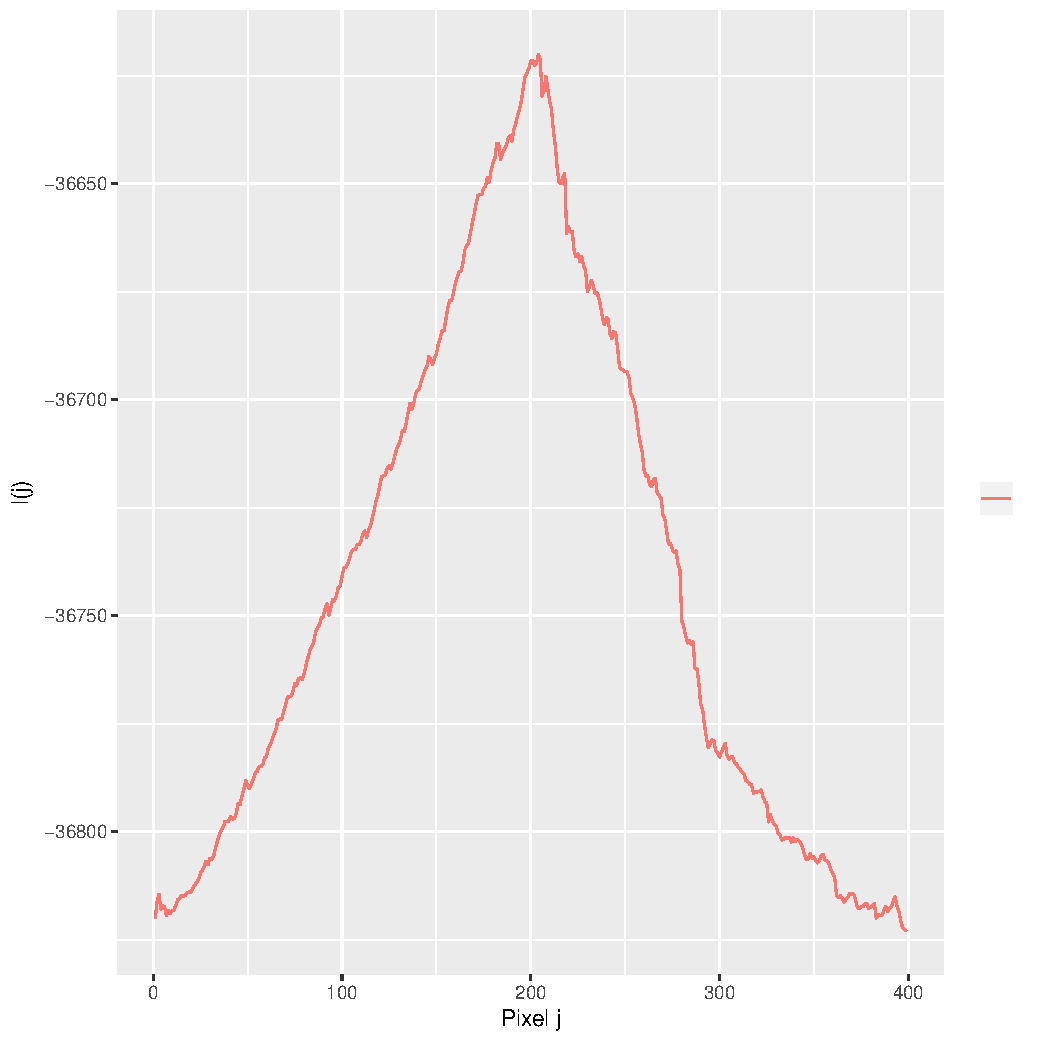
\includegraphics[width=0.32\linewidth]{grafico_l_nhfc_2014_sigmahh_artigos}}
     \subfloat[Band $\text{hv}$ \label{fig_evid_bordas:1b}]{%
       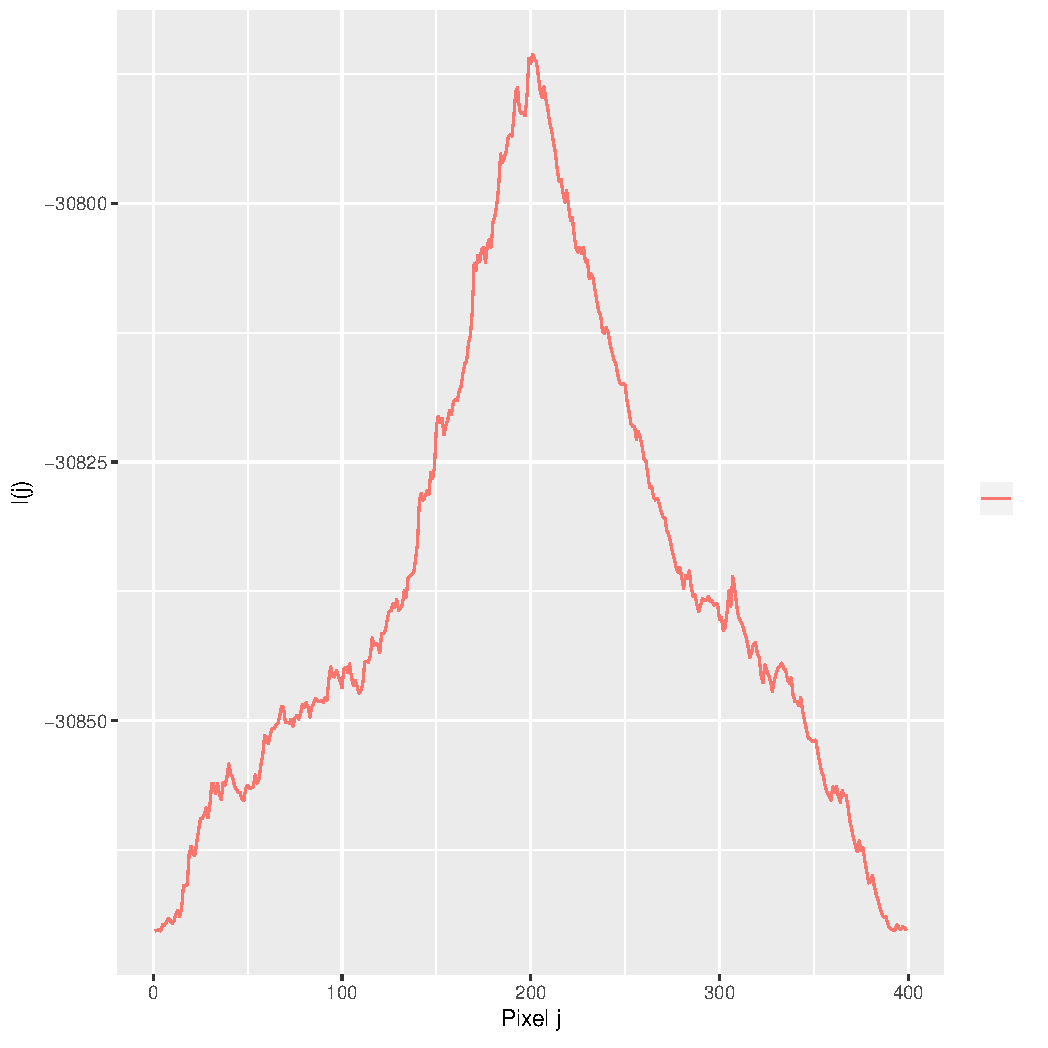
\includegraphics[width=0.32\linewidth]{grafico_l_nhfc_2014_sigmahv_artigos}}
     \subfloat[Band $\text{vv}$ \label{fig_evid_bordas:1c}]{%
       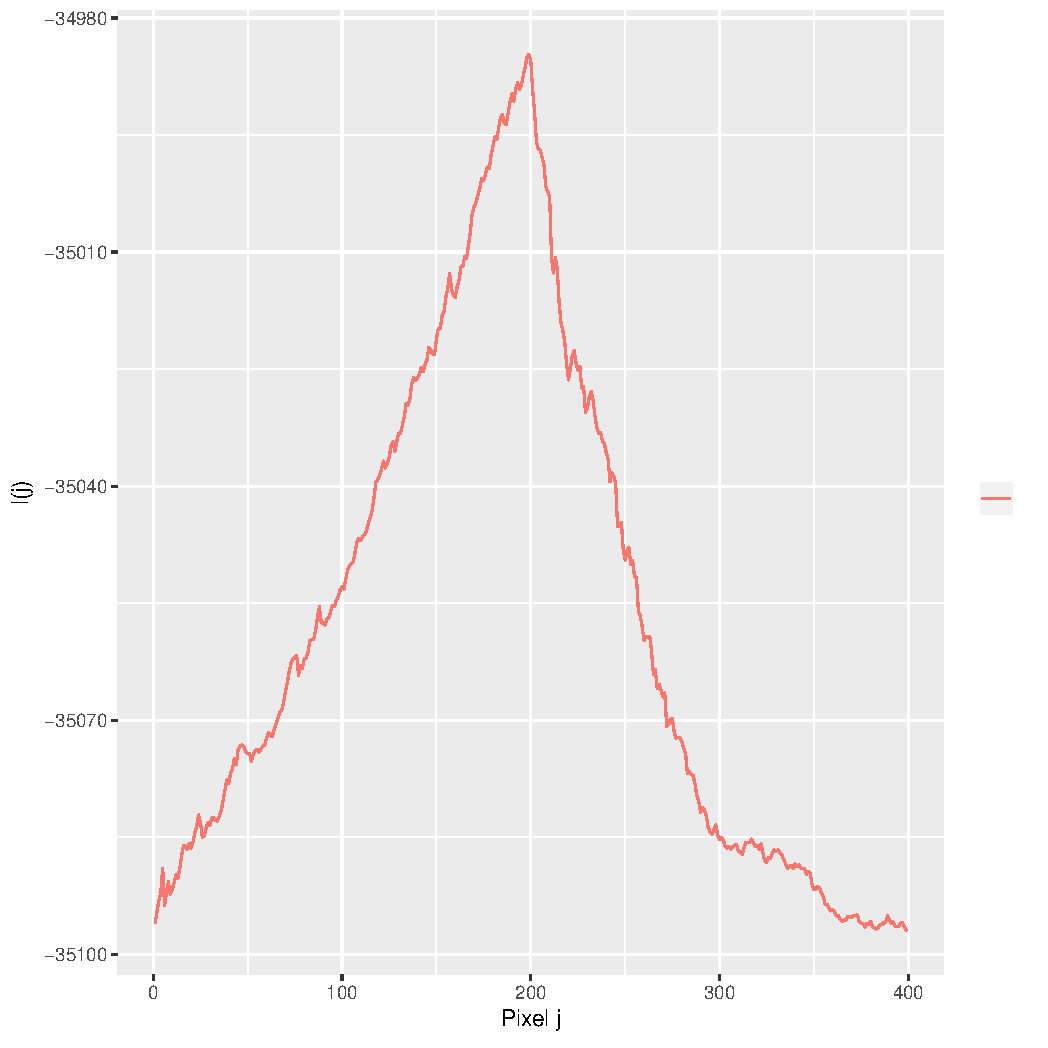
\includegraphics[width=0.32\linewidth]{grafico_l_nhfc_2014_sigmavv_artigos}}
     \caption{Edges evidences}
     \label{fig_evid_bordas}
   \end{figure}	

The functions has a peak indicating the evidence of the edge that should be captured, but the functions are not smooth, hindering the use of optimization methods that require the calculation of the derivative.
This problem was solved using Generalized Simulated Annealing (GenSA)~\cite{xgsh}, suitable for non-differentiable functions.
    
We measured the error simulating $400$ independent images and finding $\widehat\jmath$ in each line.
By construction, we consider the vertical line $200$ as the true edge in each replication, so the error for this replication is the absolute value of the difference between this point and the estimated value. 
Thus, the error for each replication is computed by $E(r) = |200 - \widehat{\jmath}(r)|$, $1\leq r \leq 400$.

We used relative frequencies to estimate the probability of having an error smaller than a number of pixels. 
Denoting $H(k)$ the number of replications for which the error is less than $k$ pixels, an estimate of this probability is $f(k)=\frac{H(k)}{400}$. 
In the tests performed in this section, $k$ varies between $1$ and $10$. 
The algorithm is described in detail in Ref.~\cite{fbgm}.
Fig.~\ref{probability_edge_detc} shows these probabilities as computed in each channel $I_\text{hh}$, $I_\text{vv}$ and $I_{vvv}$ of the image. 
  
\begin{figure}[hbt]
	\centering
	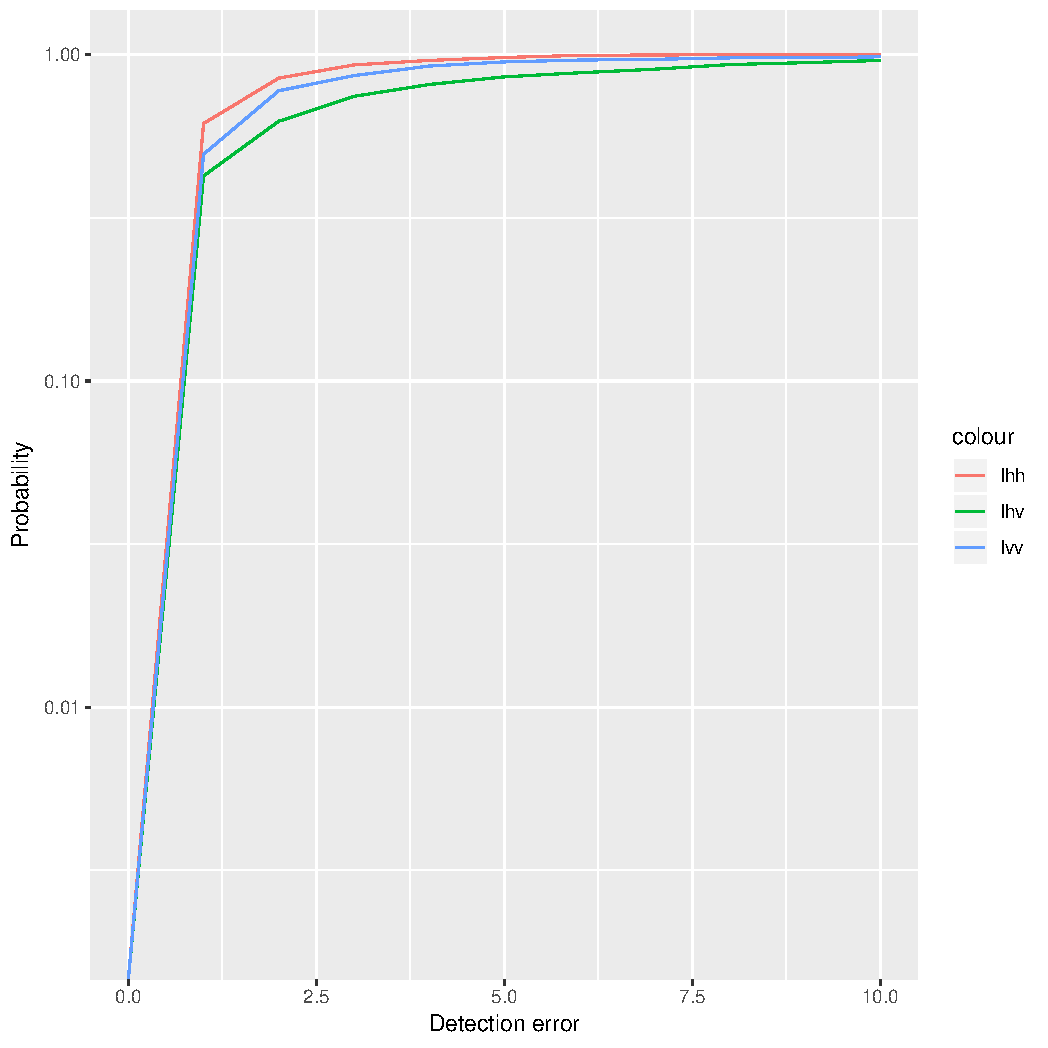
\includegraphics[width=.7\linewidth]{metricas_ihh_ivh_ivv_nhfc_artigos}%
	\caption{Probability of detecting edges evidences.}
\label{probability_edge_detc}
\end{figure}

\section{Methods of fusion of edge evidence}\label{sec_07}

\subsection{Simple average}
The simple average fusion method proposes the arithmetic mean of the edge evidence in each channel. 
The edge evidence fusion can be calculated by
\begin{equation}
	IF(x,y)=\frac{1}{nc}\sum_{i=1}^{nc}IE_i(x,y),
\end{equation}
where $nc$ is the number of channels to be used in the fusion. 
More details are presented in Ref.~\cite{mit}.

\subsection{Stationary wavelet transform -- SWT} 

This section is based on the Ref.~\cite{n_r}. SWT filters are applied separately in vertical and horizontal directions and downsampled by a factor of two in the image $I$. In this way, the image is filtered by the low pass filter $\text{L}$ and the high pass filter $\text{H}$ in the horizontal direction and then downsampled by a factor of two to create the coefficients matrices $I_\text{L}$ and $I_\text{H}$. After this, the coefficients matrices $I_\text{L}$ and $I_\text{H}$ are again subjected to the low pass and high pass filters in the vertical direction and newly downsampled by a factor of two to create sub-images. $ I_\text{LL}$,$I_\text{LH}$, $I_\text{HL}$ and $I_\text{HH}$.
The SWT fusion method can be described by the following steps:
\begin{itemize}
\item[-] calculate the SWT decomposition by getting $I_\text{HH}$, $I_\text{HL}$, $I_\text{LH}$ and $I_\text{LL}$ for each channel (image); %%% ACF O que é cada uma dessas L?
\item[-] in the decompositions $I_\text{HH}$, obtain the arithmetic mean of all channels, pixel by pixel. In the decompositions $I_\text{HL}$, $I_\text{LH}$ and $I_\text{LL}$, the maximum between each channel is found, pixel by pixel, leaving a new decomposition $\bar{L}_\text{HH}$, $\bar{I}_\text{HL}$, $\bar{I}_\text{LH}$ and $\bar{I}_\text{LL}$;
\item[-] perform the inverse SWT transformation. The image is obtained by fusing the edge evidence $IF(x,y)$.  
\end{itemize}

\subsection{Principal component analysis -- PCA}

This section is based on Refs.~\cite{n_r,mit}.
The method is comprised of the following steps:
\begin{itemize}
\item[-] organize the data in such a way that each image has a column vector, forming a $Y$ matrix of dimension $l\times nc$, where $l=m n$, the lines times the columns of the matrices to be used in the fusion;
\item[-] calculate the average of the elements of these columns, generating a vector dimension of $1\times nc$;
\item[-] subtract the average of each column from the $Y$ matrix, resulting in $X$, a matrix of the same dimension of $Y$; 
\item[-] find $C$, the covariance matrix of $X$;
\item[-] calculate its eigenvalues $\Lambda$ and eigenvectors $D$, and sort the eigenvalues and eigenvectors in descending order. The matrices generated by the eigenvalues, on the main diagonal, and the eigenvectors placed in column, have dimensions $nc\times nc$;
\item[-] compute the components $P_i={V_i}^{-1}{\sum_{i=1}^l V_i}$ with $i=1,\dots,nc$;
\item[-] fuse $IF(x,y)=\sum_{i=1}^{nc}P_iIE_i(x,y)$, recalling that $\sum_{i=1}^{nc}P_i=1$.
\end{itemize}

\subsection{ROC statistics}

The ROC method was proposed and described in detail in~\cite{gs,fawcett}:
\begin{itemize}
\item[-] obtain the evidence of edges in the channels, and store it in $E_i$ matrices, with $i=1,\dots,nc$ in a binary way;
\item[-] define a $V$ edge frequency matrix. The $V$ matrix is generated by adding the evidence of $E_i$ edges;
\item[-] use thresholds ranging from $t=1,\dots,nc$ generating $M_t$ matrices;
\item[-] compare each $M_t$, fixed with all $E_i$, find the confusion matrix to generate the ROC curve. The point of the ROC curve closest (in the sense of the Euclidean distance) to the diagnostic line will have its threshold considered optimal;
\item[-] the $M_t$ matrix which corresponds to the threshold closest to the diagnostic line is the result of the fusion.
\end{itemize}

\section{Numerical results}\label{sec_08}

We used the PolSAR image of the Flevoland region in the Netherlands, with $4$ looks, for the numerical tests. 
Fig.~(\ref{flevoland_radial_4look}) shows the region of interest, with the radial lines for edge detection.

\begin{figure}[hbt]
\centering
	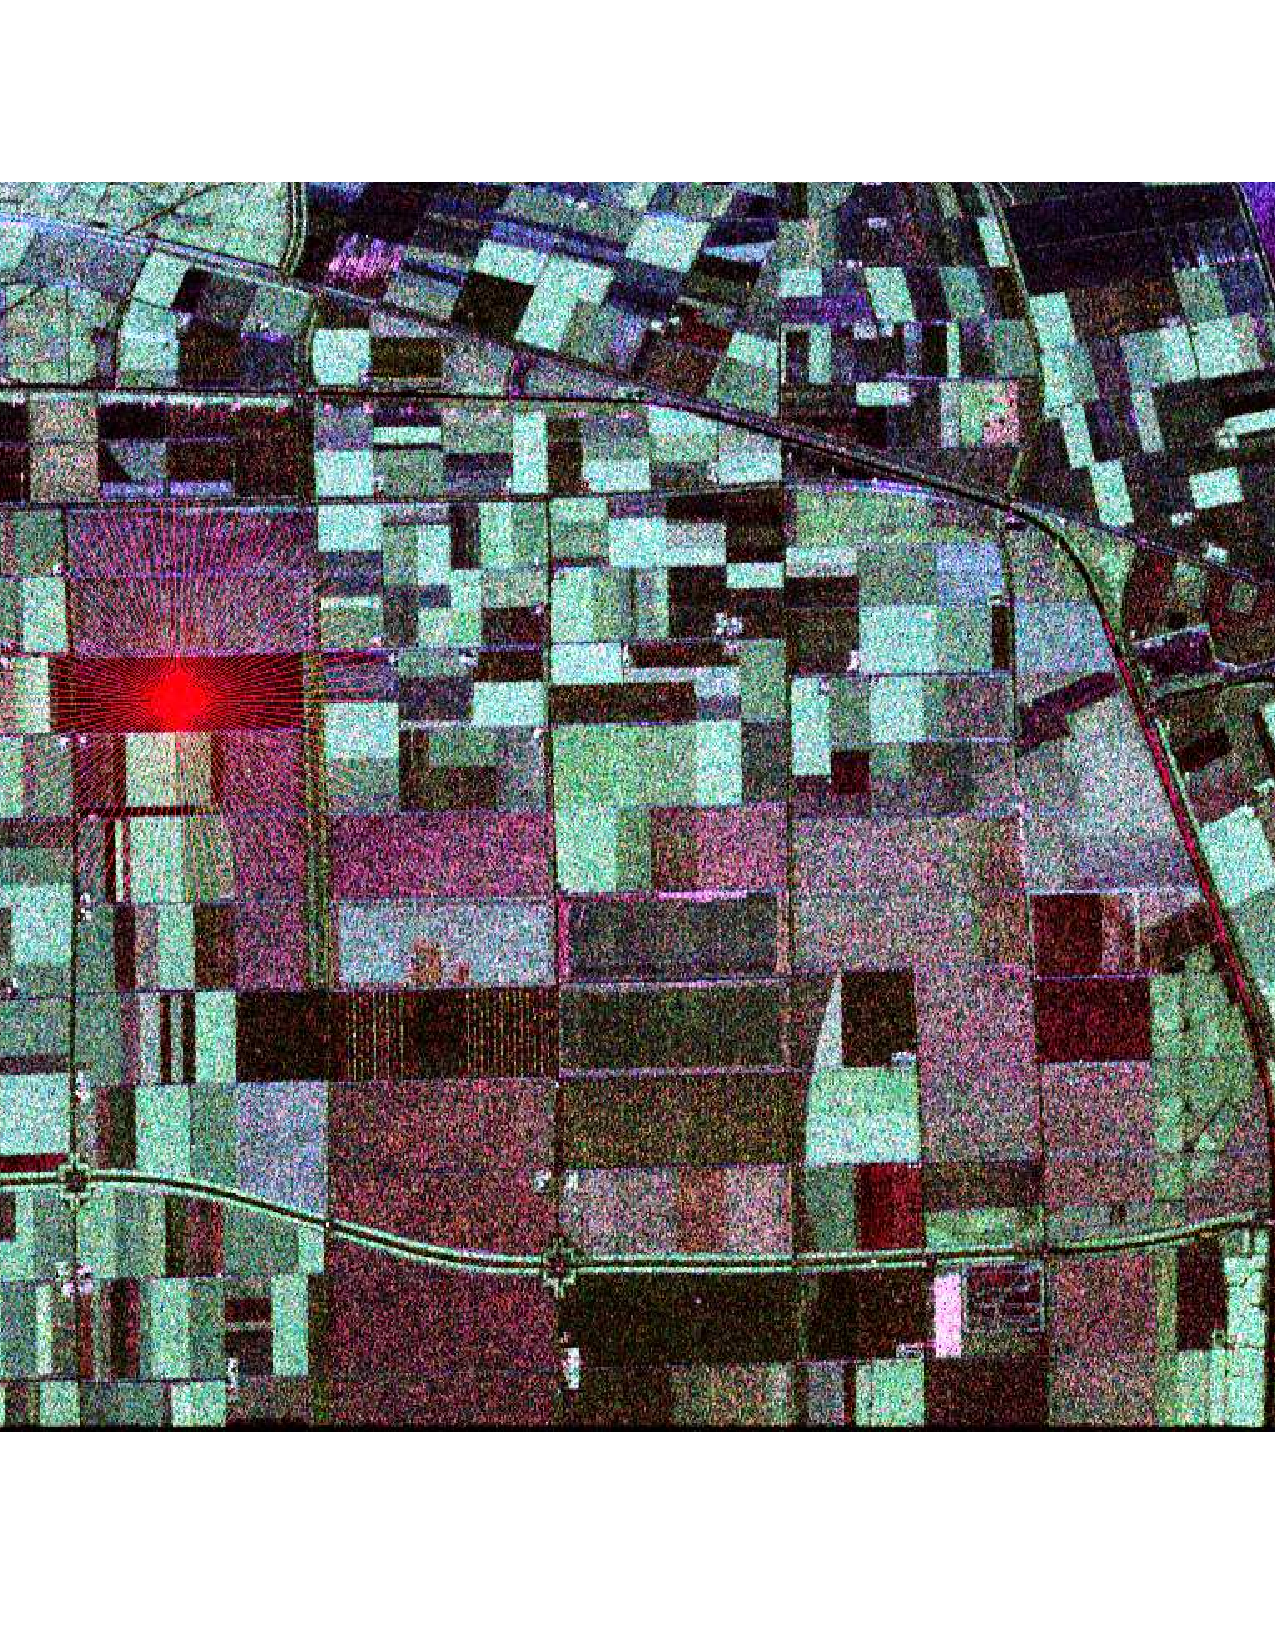
\includegraphics[width=\linewidth]{flevoland_radial_4_look}
	\caption{Region of interest (ROI) in the image of Flevoland.}
\label{flevoland_radial_4look}
\end{figure}

Figs.~\ref{evidencias_hh_hv_vv}\subref{evidencias_hh_hv_vv:a}, \subref{evidencias_hh_hv_vv:b} and~\subref{evidencias_hh_hv_vv:c} show, respectively, the edge evidence in the $\text{hh}$, $\text{hv}$ and $\text{vv}$ channels. 
The algorithm achieves better accuracy in channels $\text{hh}$ and $\text{hv}$ than in channel $\text{vv}$.  

It is noteworthy that GSaM correctly identified the maximum evidence, even in the presence of multiple local maxima as in the case of the $\text{vv}$ channel.

\begin{figure*}[hbt]
	\centering
     \subfloat[Evidences in channel $\text{hh}$ \label{evidencias_hh_hv_vv:a}]{%
       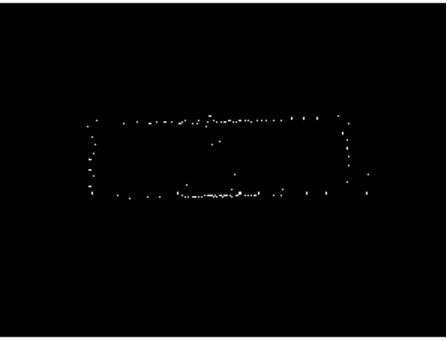
\includegraphics[width=0.32\linewidth]{flevoland_hh_evid_crop_teste}
     }
     \subfloat[Evidences in channel $\text{hv}$ \label{evidencias_hh_hv_vv:b}]{%
       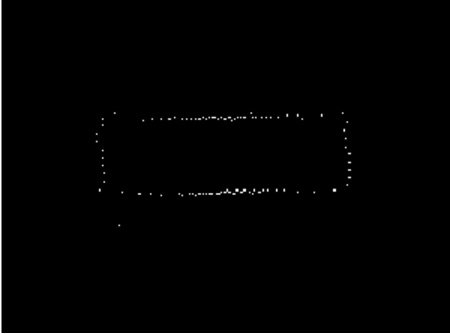
\includegraphics[width=0.32\linewidth]{flevoland_hv_evid_crop_teste}
     }
     \subfloat[Evidences in channel $\text{vv}$ \label{evidencias_hh_hv_vv:c}]{%
       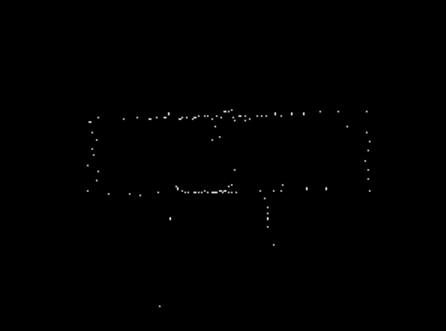
\includegraphics[width=0.32\linewidth]{flevoland_vv_evid_crop_teste}
     }
     \caption{Edges evidences}
     \label{evidencias_hh_hv_vv}
   \end{figure*}

Figs.~\ref{fusion_met}\subref{fusion_met:a}, \subref{fusion_met:b}, \subref{fusion_met:c}, and~\subref{fusion_met:d} show, respectively, the results of fusing these evidences. 

The methods shown in Figs.~\ref{fusion_met}\subref{fusion_met:a}, \subref{fusion_met:b}, \subref{fusion_met:c} and~\subref{fusion_met:d} use all the pixels detected in the three channels by using different weights: 
the average weights the pixels equally, SWT finds the coefficients of the linear combination of its wavelet bases, and PCA weights by the eigenvalues of the covariance matrix.

The ROC statistics method does not use all pixels of the channels, because the method is based on thresholds for discarding pixels. 
This was observed in Fig.~\ref{fusion_met}\subref{fusion_met:d}.

\begin{figure*}[hbt]
	\centering
     \subfloat[Average fusion\label{fusion_met:a}]{%
       %\includegraphics[width=0.2\textwidth]{example-image-a}
       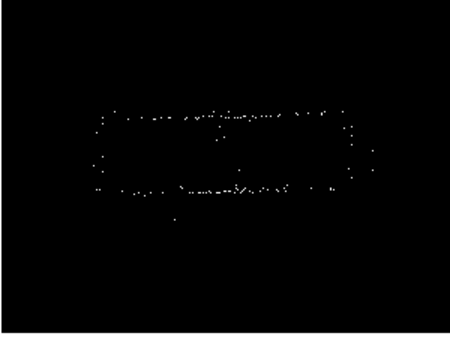
\includegraphics[width=0.32\linewidth]{flevoland_fusao_media_crop_teste}
     }
     \subfloat[SWT fusion\label{fusion_met:b}]{%
       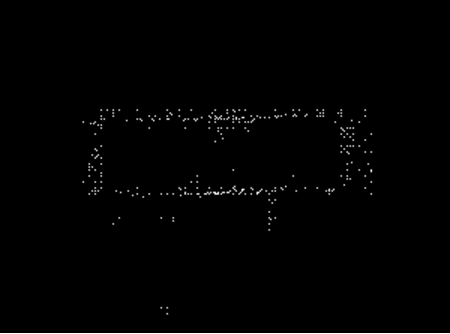
\includegraphics[width=0.32\linewidth]{flevoland_fusao_swt_crop_teste}
     }
     \subfloat[PCA fusion \label{fusion_met:c}]{%
       %\includegraphics[width=0.2\textwidth]{example-image-a}
       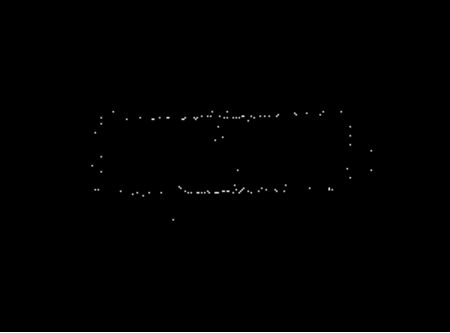
\includegraphics[width=0.32\linewidth]{flevoland_fusao_pca_crop_teste}       
     }\\
     \subfloat[ROC fusion\label{fusion_met:d}]{%
       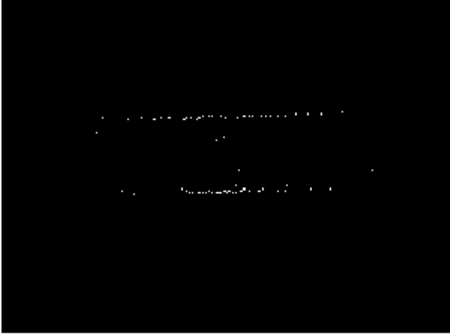
\includegraphics[width=0.32\linewidth]{flevoland_fusao_roc_crop_teste.pdf}
     }
     \caption{Fusion methods}
     \label{fusion_met}
\end{figure*}

\section{Conclusion}\label{sec_09}

In this article, we analyzed methods of fusion of edges evidence in Polsar images. 
First, we found the edges evidence using the method of maximum likelihood in the three intensities channels. 
Secondly, we applied fusion methods: simple average, SWT, PCA, and ROC curve. 
We used a simulated image to quantify and compare the results. 

The detection was performed by maximum likelihood, in which the function is not smooth and presents many local minima.
Therefore, we stress the difficulty of using classical optimization methods. 
To solve the problem, we applied Simulated Annealing because it is appropriate to optimize non-differentiable functions.

We measured the quality of the fusion with the probability of detecting correctly the edge.
We observed excellent performance in detecting evidence of edges in the intensity channels.

From the obtained results, we identified the viability of increasing the number of channels used for edge evidence detection, paving the way to research new fusion methods in PolSAR image.

\bibliographystyle{IEEEtran}
\bibliography{../../../Misc/bibliografia}
\end{document}
